\documentclass[11pt]{article}
\usepackage{fullpage}
\usepackage{hyperref}


\usepackage[english]{babel}
\usepackage[latin1]{inputenc}

\usepackage{times}
\usepackage[T1]{fontenc}

\usepackage{color}
\usepackage{colortbl}
%\usepackage{graphicx}
\usepackage{alltt}
\usepackage{marvosym}
\usepackage{pgf}
\usepackage{tikz}
%\usetikzlibrary{arrows,snakes,backgrounds}

\tikzstyle{element}=[rectangle,draw=black,fill=black!20,minimum size=1cm]
\tikzstyle{emptyel}=[rectangle,draw=black,fill=white,minimum size=1cm]
\tikzstyle{ghostel}=[rectangle,draw=white!20,fill=white!20,minimum size=1cm]
\tikzstyle{vertex}=[circle,draw=blue!50,fill=blue!20,minimum size=1cm]

%\setbeamercolor{highback}{bg=yellow}
%\setbeamercolor{nighnone}{}

\newcommand{\high}[1]{\alert<.>{#1}}
\newcommand{\highin}[2]{\alert<#1>{#2}}
\newcommand{\ithi}[1]{\item \alert<.>{#1}}
\newcommand{\rahi}[1]{\item[$\rightarrow$] \alert<.>{#1}}
\newcommand{\Rahi}[1]{\item[$\Rightarrow$] \alert<.>{#1}}
\newcommand{\qa}[5]{\only<#1>{#2}\only<#3>{#4}}
\newcommand{\tinyh}[1]{#1}

% Style definition file generated by highlight 2.13, http://www.andre-simon.de/ 

% Highlighting theme definition: 

\newcommand{\hlstd}[1]{\textcolor[rgb]{0,0,0}{#1}}
\newcommand{\hlnum}[1]{\textcolor[rgb]{0.16,0.16,1}{#1}}
\newcommand{\hlesc}[1]{\textcolor[rgb]{1,0,1}{#1}}
\newcommand{\hlstr}[1]{\textcolor[rgb]{1,0,0}{#1}}
\newcommand{\hldstr}[1]{\textcolor[rgb]{0.51,0.51,0}{#1}}
\newcommand{\hlslc}[1]{\textcolor[rgb]{0.51,0.51,0.51}{\it{#1}}}
\newcommand{\hlcom}[1]{\textcolor[rgb]{0.51,0.51,0.51}{\it{#1}}}
\newcommand{\hldir}[1]{\textcolor[rgb]{0,0.51,0}{#1}}
\newcommand{\hlsym}[1]{\textcolor[rgb]{0,0,0}{#1}}
\newcommand{\hlline}[1]{\textcolor[rgb]{0.33,0.33,0.33}{#1}}
\newcommand{\hlkwa}[1]{\textcolor[rgb]{0,0,0}{\bf{#1}}}
\newcommand{\hlkwb}[1]{\textcolor[rgb]{0.51,0,0}{#1}}
\newcommand{\hlkwc}[1]{\textcolor[rgb]{0,0,0}{\bf{#1}}}
\newcommand{\hlkwd}[1]{\textcolor[rgb]{0,0,0.51}{#1}}
\definecolor{bgcolor}{rgb}{1,1,1}



%% Uncomment this, if you want the table of contents to pop up at
%% the beginning of each subsection:
%\AtBeginSubsection[]
%{
%  \begin{frame}<beamer>{Outline}
%    \tableofcontents[currentsection,currentsubsection]
%  \end{frame}
%}

% If you wish to uncover everything in a step-wise fashion, uncomment
% the following command: 

%\beamerdefaultoverlayspecification{<+->}

% If you have a file called "university-logo-filename.xxx", where xxx
% is a graphic format that can be processed by latex or pdflatex,
% resp., then you can add a logo as follows:

% \pgfdeclareimage[height=0.5cm]{university-logo}{university-logo-filename}
% \logo{\pgfuseimage{university-logo}}


\newcommand{\anders}{Anders Jonsson}
\newcommand{\email}{\texttt{anders.jonsson@upf.edu}}

\newcommand{\ddate}{2010-2011}
\newcommand{\Cpp}{{\tt C++}}

\newcommand{\compcpp}[3]{\item{\high{#1} \begin{itemize} \item[ObjC] #2 \item[C++] #3\end{itemize}}}
\newcommand{\hashinc}[1]{\#include\textless #1\textgreater}
%\newcommand{\jfinc}[1]{{\tiny\verbatiminput{src/#1}}}   % this can be switched to \tiny\input .tex if highlight works
\newcommand{\jfinc}[1]{{\tiny\input{#1}}}

\usepackage{amssymb}
\usepackage{mathtools}
\usepackage{amsthm}
\usepackage{multirow}
\usepackage{pgfplots}
\usepackage{tikz}
\usetikzlibrary{decorations.text}
\usetikzlibrary{bayesnet}

\usetikzlibrary{arrows,automata,positioning}
\usetikzlibrary{shapes.multipart}
\usetikzlibrary{decorations.markings}
\usetikzlibrary{decorations.pathreplacing}
\usetikzlibrary{intersections, pgfplots.fillbetween}

\setlength{\textheight}{11.00in}
\setlength{\topmargin}{-0.2in}

\title{
\vspace{-1.2cm}
Machine Learning 2021-22\\ Final Exam}
\author{14 December 2021}
\date{Name: \dotfill}% NIA: \dotfill}

\newcounter{marks}
\setcounter{marks}{0}

\def\ci{\perp\!\!\!\perp}

\begin{document}

\maketitle

\newcounter{PreguntaCounter}

\begin{list}{{\bf Question \arabic{PreguntaCounter}:}}
	{\usecounter{PreguntaCounter}
	}

\item
\fbox{2 points}
\addtocounter{marks}{2}
Show that the two univariate functions $e^x$ and $x\log x$ are convex for $x>0$.\\
Hints: $\frac \partial {\partial x} e^x = e^x$, $\frac \partial {\partial x} \log x = \frac 1 x$, $\frac \partial {\partial x} x^p = p \cdot x^{p-1}$, and $\frac \partial {\partial x} \left( f(x) \cdot g(x) \right) = \frac {\partial f(x)} {\partial x} \cdot g(x) + f(x) \cdot\frac {\partial g(x)} {\partial x}$.

\framebox[16cm][l]{ 
\parbox{15.9cm}{
\vspace*{7cm}
}}

\item
\fbox{2 points}
\addtocounter{marks}{2}
Solve the following constrained optimization problem:
  \begin{align*}
	\max_{x,y} \; & xy\\
	\mathrm{s.t.} \; & x + 2y = 1
  \end{align*}
  Indicate the optimal value of $x$ and $y$ as well as the optimal value of the objective.

\framebox[16cm][l]{ 
\parbox{15.9cm}{
\vspace*{7cm}
}}

\pagebreak



\item
\fbox{1 point}
\addtocounter{marks}{1}
Which is the objective of $k$-means clustering? How does the $k$-means algorithm approximate a solution to this objective?

\framebox[16cm][l]{ 
\parbox{15.9cm}{
\vspace*{6.2cm}
}}


\item
\fbox{1 point}
\addtocounter{marks}{1}
Describe the process of using validation to perform model selection. Why is the validation loss an optimistic estimate of the true loss?

\framebox[16cm][l]{ 
\parbox{15.9cm}{
\vspace*{6.2cm}
}}

\item
\fbox{1 point}
\addtocounter{marks}{1}
Three popular models for supervised learning are decision trees, support vector machines, and neural networks. For each of these three models, list one advantage and one disadvantage.

\framebox[16cm][l]{ 
\parbox{15.9cm}{
\vspace*{6.2cm}
}}


\pagebreak

Name: \dotfill

\item
\fbox{1 point}
\addtocounter{marks}{1}
Briefly explain the backpropagation algorithm, and describe how the algorithm can be efficiently implemented.

\framebox[16cm][l]{
\parbox{15.9cm}{
\vspace*{6.2cm}
}}

\item
\fbox{1 point}
\addtocounter{marks}{1}
Explain how a convolutional layer works in deep learning. How are convolutional layers implemented in practice? What changes do we have to make to standard backpropagation?

\framebox[16cm][l]{ 
\parbox{15.9cm}{
\vspace*{6.2cm}
}}


\item
\fbox{2 points}
\addtocounter{marks}{2}
Describe qualitatively in what consists the mechanism called \emph{attention} in deep learning and how attention is integrated in the Transformer network.
You can help yourself with a diagram.

\framebox[16cm][l]{ 
\parbox{15.9cm}{
\vspace*{6.2cm}
}}


\pagebreak

Name: \dotfill

\item
\fbox{1 point}
\addtocounter{marks}{1}
A Bayesian network models the relation between the variables oil ($oil$), inflation ($inf$), economy health~($eh$), British petroleum stock price ($bp$), and retailer stock price ($rt$).
\begin{figure}[!th]
\begin{center}
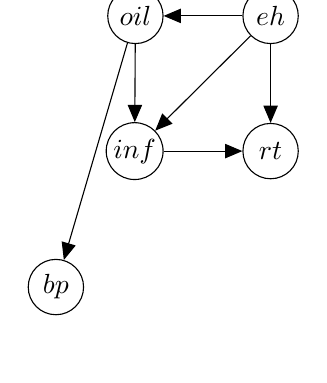
\begin{tikzpicture}
  % Define nodes
  \node[latent]             (oil) {$oil$};
  \node[latent, right=of oil]             (eh) {$eh$};
  \node[latent, below=of eh]              (rt) {$rt$};
  \node[latent, left=of rt]            (inf) {$inf$};
  \node[latent, below=of inf, xshift=-1cm]   (bp) {$bp$};
  % Connect the nodes
  \edge {eh} {oil} ; %
  \edge {oil} {inf} ; %
  \edge {eh} {rt} ; %
  \edge {inf} {rt} ; %
  \edge {eh} {inf} ; %
  \edge {oil} {bp} ; %
  \end{tikzpicture}
 \caption{A simple Bayesian network}\label{fig:oil}
\end{center}
\end{figure}
\vspace{-1cm}
   \begin{enumerate}
    \item Write down the corresponding factorization of the joint probability distribution.
    \item Use the D-Separation algorithm to determine whether the following conditional independences.
\begin{enumerate}
\item Is $eh$ independent of $bp$ if no evidence is provided? Why?
\item Is $eh$ independent of $bp$ if we observe that the $oil$ is $high$? Why?
\item Is $rt$ independent of $bp$ if we observe that $eh$ is $low$? Why?
\end{enumerate}
\end{enumerate}
\framebox[16cm][l]{ 
\parbox{15.9cm}{
\vspace*{4.5cm}
}}

\item
\fbox{1 point}
\addtocounter{marks}{1}
We acquire data $\mathcal{D}$ consisting of $N$ independent and identically distributed samples $x_i, i = 1,\hdots,N$ at different times.
We assume a Gaussian generative model for $\mathcal{D}$ with constant variance $\sigma^2$ and mean determined by the output of a time-dependent model $F_{\boldsymbol{\theta}}(t)$ with parameters $\boldsymbol{\theta}$.
\vspace{-.2cm}
\begin{enumerate}
\item Write down the formula for the corresponding likelihood function of $\boldsymbol{\theta}$ for fixed $\mathcal{D}$.
\item Explain how Bayes theorem can be used to update the parameters $\boldsymbol{\theta}$ in light of $\mathcal{D}$.\\
\end{enumerate}
\vspace{-.6cm}
Hint: A Gaussian distributed variable $y$ with mean $\mu$ and variance $\sigma^2$ has density $f(y)=\frac{1}{\sigma\sqrt{2\pi}}e^{-\frac{1}{2}\left(\frac{y-\mu}{\sigma}\right)^2}.$

\framebox[16cm][l]{ 
\parbox{15.9cm}{
\vspace*{5cm}
}}


\end{list}


\end{document}
